%*************************************************************************
% Chapter 1
%*************************************************************************


\chapter{Einleitung}
\label{ch:intro}
The topic of polystores has been an active area of research for more than ten years. 
This is relatively easy to explain, as the digital world is becoming increasingly multifaceted and complex. 
The amount of data to be processed continues to grow. 
Whereas the goal used to be to design and implement database concepts that used storage space as sparingly as possible, 
the focus today tends to be on performance. 
Recommendation systems must be able to provide meaningful suggestions in real-time 
or very quickly based on inputs, for example in the context of 
a customer $\mathbf{C}$ bought item $\mathbf{A}$, then they also bought item $\mathbf{B}$ or item $\mathbf{C}$ or $\ldots$
:
\[
\forall c \in \mathcal{C} \quad \Bigl( \text{Bought}(c, A) \implies \bigl( \text{Bought}(c, B) \lor \text{Bought}(c, C) \lor \cdots \bigr) \Bigr)
\]
The topic of polystores has been an active area of research for more than ten years. 
Such a request can only be meaningfully and efficiently answered if a suitable algorithm quickly receives input from an appropriate database. 
Such a database could be, for example, a graph database. 
In a web shop, for instance, where such a recommendation system is implemented, typical database transactions, 
known as Create, Read, Update, Delete (CRUD) operations, frequently occur. 
These transactions can often be better handled by a classical SQL database.
Such a system can be referred to as a polystore because it requires at least two different database systems 
or data stores to function efficiently. 
Sometimes, the transitions are more fluid than in the aforementioned example of an e-commerce system 
with one database for the recommendation engine and another for the transactional part of the system. 
For example, so-called data streams can be handled just as well in a document-based database as classical CRUD operations. 
It is conceivable that both parts of a hypothetical system could be mapped using, for example, a MongoDB.

\noindent In this case, it would be sensible to measure whether a system consisting of two or more different services 
that share a data store or database system would benefit from reallocating services or datasets to a data store when 
faced with a dynamically changing workload. 
This could be beneficial, for example, if certain transactions or commits start taking more time, negatively 
impacting user experience or system performance.\newline

\noindent Fundamentally, the issue is that in a system, there must be at least two different services $\mathbf{S}$, 
each assigned to a data store $\mathbf{D}$ and having a certain workload $\mathbf{W}$. 
If the workload $\mathbf{W}$ changes or certain thresholds $\mathbf{Th}$ are exceeded, 
the services or the affected service should be assigned to another, possibly more suitable, data store $\mathbf{D}$. 
This should only happen if the service $\mathbf{S}$, in conjunction with the newly assigned data store $\mathbf{D_n}$, exhibits an improved workload
$\mathbf{W_i}$.\noindent
In summary, the situation can be described as follows:
\section*{Service Reassignment Based on Workload}

We define the following:

\begin{itemize}
    \item \textbf{Services:} 
    \[
    \mathcal{S} = \{ S_1, S_2, \ldots, S_n \} \quad (n \geq 2)
    \]
    \item \textbf{Datastores:} 
    \[
    \mathcal{D} = \{ D_1, D_2, \ldots, D_m \}.
    \]
    \item \textbf{Workload Function:} 
    \[
    W: \mathcal{S} \times \mathcal{D} \to \mathbb{R}_{\ge0},
    \]
    where \(W(S,D)\) measures the workload of service \(S\) when using datastore \(D\) (lower is better).
    \item \textbf{Thresholds:} Let \(Th \ge 0\) be the workload threshold, and let \(\epsilon > 0\) be a parameter defining a significant change in workload over time.
\end{itemize}

Let \(A: \mathcal{S} \to \mathcal{D}\) be the current assignment function, meaning that a service \(S\) is assigned to a datastore \(A(S)\).

For a given service \(S\), if either:
\[
\bigl|W(S, A(S))_t - W(S, A(S))_{t-1}\bigr| \ge \epsilon
\]
or
\[
W(S, A(S)) \ge Th,
\]
and there exists another datastore \(D' \in \mathcal{D}\) such that:
\[
W(S, D') < W(S, A(S)),
\]
then we reassign service \(S\) to \(D'\).

This rule can be written as:
\[
A'(S) =
\begin{cases}
D', & \text{if } \left( \bigl|W(S, A(S))_t - W(S, A(S))_{t-1}\bigr| \ge \epsilon \text{ or } W(S, A(S)) \ge Th \right) \\
    & \quad \text{and there exists } D' \in \mathcal{D} \text{ with } W(S, D') < W(S, A(S)); \\[1ex]
A(S), & \text{otherwise.}
\end{cases}
\]
It is therefore necessary to constantly check how a system of datasets, services, and data stores should be structured 
in order to optimally meet the requirements for this system. 
This is precisely the topic that the present work addresses.
%
% Section: Motiva
%
\section{Motivation}
\label{sec:intro:motivation}
Es existieren bislang nur wenig bis gar keine polystoren Systeme die es über den Status Prototyp
geschafft haben. Das Projet was wohl am fortgeschrittensten ist ist Polyphenie DB.
Ein Erklärungsansatz für den mangelhafte Verbreitung von Polystore Systemen und oder deren 
produktiven Einsatz ist, dass die Implmentierung immer noch schwierig und aufwendig ist.

Ein anderer Erklärungsansatz ist, dass die Vorteile eines Polystores erst zum tragen 
kommen, wenn dieses in einem dynamischen Umfeld bzw. System zum Einsatz kommt. In einem dynamischen
Umfeld ändert sich der Workload und damit ist wie bereits beschrieben die initiale oder 
aktuelle Zuordnung von Datastores zu Datasets nicht mehr valide bzw. optimal.

Nun ist es schwer vorstellbar, dass in einem produktiven Betrieb permanent manuell Datasets
anderen Datenbanken und Datenbank Systemen zugeordnet werden. Ein solcher Eingriff ist komplex,
erfordert eine sorgfältige Vorbereitung und beansprucht in den meisten Fällen einen 
nicht unerheblichen Teil der Ressourcen (insbesondere Personal wie Datenbank Administratoren und 
Backend-Entwickler etc.). Des weiteren geht mit einer solchen Umstellung ein nicht
zu unterschätendes Risiko einher. Dieses Risiko kann durch bestimmte Verfahren wie das Testen 
der Umstellung in einer gekapselten Testumgebung, einer schrittweisen Umstellung etc. minimiert 
werden, dennoch sind Anpassungen am Datenmodell bzw. an der Persistenz-Schicht eines Systems immer heikel
und unterliegen häufig einem sehr statischen Setup.

Des Weiteren stellt sich immer die Frage wenn festgestellt wird, dass eine Zuordnung Datasets zu 
Datastores nicht mehr optimal ist, was die bessere Lösung wäre und wie sich der Workload durch eine 
Unmstellung potentiell verändern würde. Eine manuelle Überprüfung der Workloads ist zwar denkbar aber schwer
mit dem Alltag von Entwicklungs-Teams vereinbar. 
Wenn man feststellt, dass die Performance aber auch andere parameter wie Verfügbarkeit, also letztendlich
Service Level Agreements (SLA) nicht mehr den Anforderungen entsprechen, stellt sich die Frage, wie 
das System umgestellt werden sollte oder umgestellt werden kann um die Anforderungen wieder 
zu erfüllen.

Die weiterführende Vision bzw. Motivation dieser Arbeit ist, eine Polystore System welches auf Basis
von Workloads, Applikationsparametern und SLA automatisch eine initial Zuordnung von Datasets zu Datastores vornimmt
und dieses Setup kontinuierlich und automatisiert überwacht und im Fall von Abweichungen 
sich selbst optimiert. Ein solches System wäre gerade für komplexe Anwendungen mit heterogenen Anforderungen
an die entsprechenden Datastores ein Mehrwert und trägt der Erkenntnis Rechnung 
das im Bereich Datastores und Datenbank eine One Fits All Lösung nicht bzw. bislang niht existiert.
So entsteht für den Benutzer ein optimiertes Nutzererlebnis und das Entwicklungs-Team kann sich voll 
auf die Implmentierung von User Interfaces und Business Logik fokussieren.

%
% Section: Ziele
%
\section{Ziele der Arbeit}
\label{sec:intro:goal}
Die Ziele der Arbeit sind wie folgt: \\

1. Einen theoretischen Überblick zu lieferen, wie ein dynamisches polystore basiertes System beschaffen 
sein muss bzw. beschaffen sein sollte, damit dieses in produktiven Umgebungen eingesetzt werden  kann.
\\

2. Konkret zu beschreiben welche Schritte ein dynamisches polystore basiertes System immer wieder durchlaufen 
muss um sich selbst aktuell zu halten und ein möglichst optimalen fit zwischen Datasets und Datastores
zu generieren.
\\
3. Einen Prototyp zu implementieren, der auf Basis von definierten Inputs eine intiale Zuordnung von 
Datasets zu Datastores herstellt. 

4. Auf Basis des Prototyp aus 3. einen Algorithmus zu implementieren, der den Workload von Datastores
analysiert und dynamisch neue Zuordnungsvorschläge generiert, wenn sich der Workload verändert.

5. Theoretisch zu beschreiben welche Schritte unternommen werden müssen, um eine dynamisch errechnete
neue Zuordnung von Datasets zu Datastores zu exekutieren.

% Section:  der Arbeit
%
\section{Gliederung}
\label{sec:intro:structure}

Die Arbeit ist wie folgt gegliedert:

Nach der Einleitung werden in Chapter2 TODO Terminologische Grundlagen die für das Verständnis
der Arbeit wichtig sind erörtert.

In Chapter3 TODO beginnt der Hauptteil der Arbeit, der sich mit den Zielen 1. und 2. aus Chapter TODO 
beschäftigt. In diesem Kapitel soll vor allem ein Überblick vermittelt werden, wie 
dynamisch polystore basiertes System funktionieren kann und welche Kernelemente und Schnittstellen 
dieses enthalten muss.

Chapter4 beschäftigt sich mit der Implmentierung der Prototypen in Verbindung mit den Zielen 4 und 5 TODO.
Es soll Konkret beschrieben werden wie der Prototyp aufgebaut ist bzw. der Algorithmus zur 
dynamischen Neuzuteilung funktioniert. Zusätzlich werden die Ergebnisse aus dem Testbetrieb beschrieben
und gegebenfalls sinnvolle Ergänzungen und oder Einschränkungen bezogen auf den praktischen Einsatz 
dokumentiert.

Chapter5 beschreibt die konkreten Schritte zur Umsetzung einer dynamischen Neuzuteilung von Datasets
zu Datastores. Wie können Schnittstellen aussehen oder müssen diese beschaffen sein um Datasets 
einen neuem Datastore zuzuweisen? Welche Rolle spielen Konzepte wie Objekt Relationale Mapper (ORM)?
Welche konkreten Arbeitsschritte müssen durchlaufen wie durchlaufen werden um die neue Zuordnung
so umzusetzen, dass die zu Grunde liegende Anwendung oder das zu Grunde liegende System weiter 
arbeitsfähig ist? Welche Service Level Agreements müssen wie eingehalten werden und was bedeuten
zum Beispiel Anforderungen wie eine Zero Downtime für ein solches System?

In Chapter 6 werden die Ergebnisse aus dem Hauptteil (TODO Chapter3 bis Chapter5) zusammengefasst.
Zusätzlich soll ein Ausblick gegeben und Empfehlungen gegeben werden, wie das Thema dynamische 
Polystores weiter entwickelt werden können.
Die Arbeit endet mit einem Fazit bezogen auf die zusammengefassten Ergebnisse und den Ausblick.


%*************************************************************************
% Chapter 2
%*************************************************************************


\chapter{Terminologische Grundlagen}
Nach der Einleitung sollen nun in diesem Kapitel wichtige Terminologische Grundlagen geklärt werden,
um ein einheitliches Verständnis zu generieren.

Dataset

A dataset is a structured collection of related data that is organized for efficient storage, retrieval, and analysis. 
In the context of datasets and datastores, it typically refers to:

Organization: Data arranged in a systematic format (e.g., tables, files, or arrays) that can be easily queried or processed.\newline
\\
Purpose: Aimed at supporting tasks like analysis, reporting, or machine learning model training.\newline
\\
Metadata: Often accompanied by metadata that describes the structure, source, and meaning of the data, enhancing its usability. \newline
\\
Storage: May be stored in various datastores such as databases, file systems, or cloud storage services, ensuring accessibility and scalability.

Datastore

A datastore is a system or repsitory designed for the storage, management, and retrieval of data, including datasets and other data objects. In the context of datasets and datastores:

Storage Mechanism: A datastore provides the underlying nfrastructure to physically or logically store data. This can be implemented as a database, file system, data warehouse, or cloud storage service\newline
\\
    Management and Retrieval: It offers methods for efficiently accessing, querying, and updating the stored data. This might involve indexing, transaction management, or specialized query languages.
\\
    Data Integrity and Security: Datastores often include mechanisms for ensuring data accuracy, consistency, and protection against unauthorized access.
\\
    Scalability: They are built t handle varying amounts of data, supporting growth and high performance as data volume increases.
\\

Datasets and Datastores\\

In summary, while a dataset is the structured collection of data used for analysis or processing, 
a datastore is the system that houses and manages these datasets, ensuring that data is organized, accessible, and secure.

Nach dem die grundsätzlichen Begriffe Datasets und Datastores geklärt sind, werden die beiden Begriffe Mulltistore und 
Polyglot Persistenz definiert und voneinander abgegrenzt. Beide Konzepte honorieren, dass eine One Size fits all Lösung für 
verschiedenartige Datassets nicht existiert und pro Dataset er jeweils best passende Datastore genutzt werden sollte.


Multistore

Ein Multistore besteht aus einer einzigen öffentlichen Schnittstelle und übersetzt die Anfragen an diese 
Schnittstelle zu Query Interface der verschiedenen und verschiedenartigen Datastores Dij wobei i den jeweiligen Datastore
identifiziert und j den Typ des Datastores abbildet:

\begin{figure}[htbp]
    \centering
    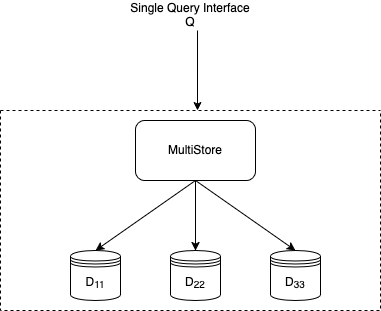
\includegraphics[width=0.60\textwidth]{gfx/examples/master_thesis-multistore.png}
    \caption{Concept of a Multistore}
    \label{fig:multistore}
\end{figure} 


Polyglot Persistenz
Ein Polystore wiederum bietet verschiedene öffentliche Schnittstellen Q1,...,QN und leitet die Anfragen an die entsprechenden 
Datastores 1,...,N weiter.

\begin{figure}[htbp]
    \centering
    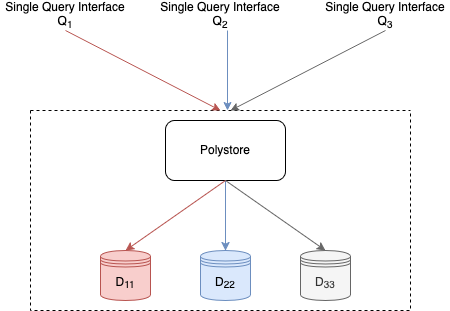
\includegraphics[width=0.60\textwidth]{gfx/examples/master_thesis-polystore.png}
    \caption{Concept of a Multistore}
    \label{fig:multistore}
\end{figure} 

Polystore
Ein Polystore ist eine Kombination aus Multistore und Polyglot Persistenz.

%*************************************************************************
% Chapter 3
%*************************************************************************

\chapter{Initiale Zuordnung von Datasets zu Datastores}

Nach der Klärung wesentlicher Begriffe und Terminologien beginnt nun im Chapter3 der Hauptteil
der Arbeit. Dieser beginnt mit der initialen Zuordnung von datasets zu Datastores.
Es wird im weiteren von einem Zustand auf der so genannten grünen Wiese ausgegangen.
Das heißt eine beliebige Applikation bzw. System wurde entwickelt und soll nun 
deployed bzw. bereitgestellt werden. Hierfür ist es notwendig, dass die initiale
Zuordnung von datasets zu datastores feststeht.
Grundsätzlich ist also festzuhalten, dass der initale Zuordnungsprozess 
optimalerweise in eine Deployment Pipeline eingebunden wird.
Ein Vorteil dieser Vorgehensweise ist, dass die gemachte Zuordnung über ein 
Staging-System getestet werden kann.

\section{Initiale Zuordnung von Datassets zu Datastores}
\label{sec:main:init}
In diesem Kapitel wird der Arbeitsschritt des Programms die initiale Zuordnung von Datasets
zu Datastores beschrieben. In Kapitel TODO wird der grundsätzliche Aufbau des Systems,
referenzierend auf die Beschreibung aus Kapitel TODO beschrieben. \newline
In Kapitel TODO wird der o.g. erste Arbeitsschritt praktisch beschrieben, also die 
konkrete Implmentierung eines Programms für die intiale Zuordnung, eingebettet in das
in dem vorangegangenen Kapitel TODO beschriebene Gesamtsystem.
\newpage
\subsection{Aufbau des Gesamtsystems}
\label{subsec:main:init:system}
Der Abbildung \ref{fig:architecture} ist der Aufbau des Gesamtsystems zu entnehmen:

\begin{figure}[htbp]
    \centering
    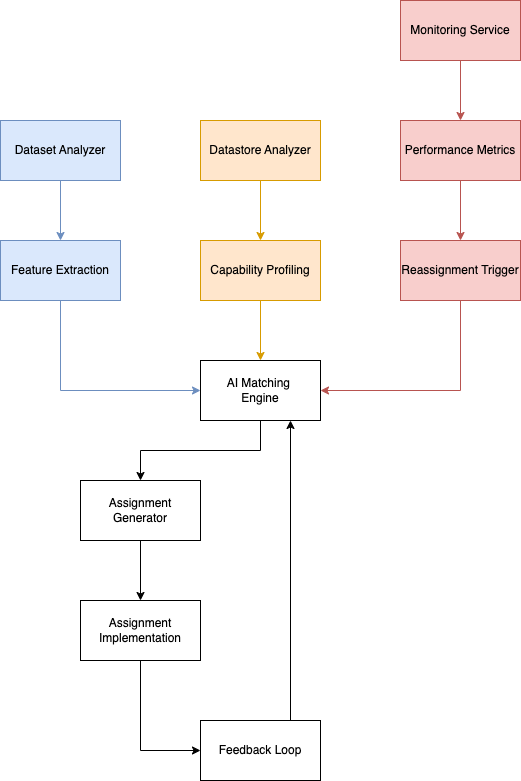
\includegraphics[width=0.60\textwidth]{gfx/examples/master_thesis-architecture.png}
    \caption{System Architecture}
    \label{fig:architecture}
\end{figure} 

Das Gesamtsystem bzw. dessen Architektur kann in verschiedene Module eingeteilt werden.
\subsubsection{Dataset Analysis Module}
\label{ssubsec:main:init:system:dam}
Das erste Modul ist das Dataset Analysis Module (DAM). Das DAM (blaue Färbung in \ref{fig:architecture})
hat die folgenden drei Hauptaufgaben:
\begin{description}
    \item[Feature Extraction:] Analyse von eigehenden Datasets um relevante Features zu extrahieren.
    \item[Determine Datatypes:] Determines datatypes, structure, size, access patterns, query frequency. 
    \item[Feature Vector:] Creation a of feature vector for each dataset. 
\end{description}
Zusammenfassend kann man sagen, dass das DAM Datassets als Input entgegennimmt und diese klassifiziert.
\subsubsection{Datastore Profiler}
\label{ssubsec:main:init:system:dp}
Das nächte Modul ist der Datastore Profiler (DP, oranger Bereich in \ref{fig:architecture}). Die Hauptaufgaben des DP sind die folgenden:
\begin{description}
    \item[Katalogisierung von Datastores:] Catalogs available datastores with their capabilities.
    \item[Performance Messung:] Measures performance characteristics for different data types
    \item[Datastore Capability Matrix:] Creation and maintenance of Capability Matrix for each Datastore. 
\end{description}
Zusammenfassend ist der DP dafür verantwortlich alle verfügbaren Datastores zu katalogisieren und 
eine Matrix zu erstellen und zu warten, derer man die entsprechenden Fähigkeiten aber auch 
umgekehrt auch deren Limitationen entnehmen kann.

\subsubsection{Dynamic Reassignment Module}
\label{ssubsec:main:init:system:drm}

Das Dynamic Reassignment Module (DRM, roter Bereich in \ref{fig:architecture}) monitort das zugrunde liegende Gesamtsystem 
aus Datasets und Datastores.
Als Input erhält das DRM System Conditions und Performance Metrics.
Auf Basis des oben genannten Inputs werden Veränderungen dedektiert und reassignment getriggert, werden entsprechende
Grenzwerte über- oder unterschritten werden. 
Kompakt sind die drei Hauptfunktionen des DRM die folgenden
\begin{description}
    \item[System Monitoring:] Monitoring of system conditions and performance metrics.
    \item[Change Detection:] Detection of changes that warrant reassignment, based in thresholds.
    \item[Datastore Capability Matrix:] Triggers reassignments with minimal disruption. 
\end{description}

\subsubsection{AI Matching Engine}
\label{ssubsec:main:init:system:ame}
Das dritte Modul ist die AI Matching Engine (AME). Die AME ist dafür verantwortlich, 
den Input aus dem DAM (\ref{ssubsec:main:init:system:ame}), dem DP (\ref{ssubsec:main:init:system:dp})
und dem DRM (\ref{ssubsec:main:init:system:drm}) um Datassets zu Datastores zuzuordnen.

\subsection{System Input parameters}
\label{subsec:main:init:input}
Nach dem die Architektur des Gesamtsystems im Kapitel \ref{subsec:main:init:system} erklärt wurde, sollen nun 
für das System relevante Inputparamter beschrieben werden.

\subsubsection{Dataset related Input}
\label{ssubsec:main:init:input:dataset}

Bezogen auf Datasets sind im wesentlichen die folgenden parameter von entscheidener Bedeutung:
\begin{description}
    \item[Data structure]: Cluster structured versus unstructured data and schema complexity.
    \item[Size]: Current size and growth rate of the dataset.
    \item[Access patterns]: Read-heavy versus write-heavy usage of the dataset.
    \item[Query complexity]: Cluster simple lookups versus complex analytics.
    \item[Consistency Requirements]: Cluster strong versus eventual consistency.
    \item[Latency Requirements]: Evaluate the needed response time.
    \item[Datas Relationships]: Check for connections to other datasets.        
\end{description}
Auf die einzelnen Inputs wird ab dem Kapitel TODO im Detail eingegangen. 
Nach der Aufzählung der Dataset bezogenen Input parameter, werden nun die Input parameter
bezogen auf Datastores aufgezählt.

\subsubsection{Datastore related Input}
\label{ssubsec:main:init:input:datastore}
Für die Beurteilung ob ein Dataset mit entsprechenden Kriterien (Vergleiche Chapter \ref{ssubsec:main:init:input:dataset})
zu einem potentiellen Datastore passt, ist eine hinreichende Beschreibung der Beschaffenheit und der characteristics
der zur Verfügung stehenden Datastores erforderliche. Nachfolgend werden die Kriterien aufgezählt die in der 
vorliegenden Arbeit Berücksichtigung finden. An dieser Stelle sei erwähnt, dass die Inputparameter für 
Datassets (Chapter \ref{ssubsec:main:init:input:dataset}) aber auch die parameter bezogeb auf Datastores
noch erweitert werden können.
Datastore bezogenene für diese Arbeit relevante Inputparameter sind die folgenden:
\begin{description}
    \item[Type of Datastore]: A distinction is made between Relational, document, key-value, graph based datastores.
    \item[Performance profile]: Evaluation of the datastore related speed characteristics.
    \item[Cost model]: Storage and operation costs of the related datastore.
    \item[Scalability]: Horizontal and vertical scaling capabilities of the related datastore.   
\end{description}




%*************************************************************************
% Chapter 4
%*************************************************************************

\chapter{Dynamische Allokation und Re-Allokation von Datasets zu Datastores}


%*************************************************************************
% Chapter 5
%*************************************************************************

\chapter{Datenmodell und Datenbankseitige Umsetzung von Datastore Re-Allokationen}

%*************************************************************************
% Chapter 6
%*************************************************************************

\chapter{Schlussbetrachtung}